% Author = warrior
% Date = 26/5/21

% Definitionsprojectestructure

%\documentclass{article}

% Links
% https://latex-tutorial.com/tutorials/
% https://robjhyndman.com/hyndsight/indexing-in-latex/
% https://es.overleaf.com/learn/latex/Headers_and_footers
% https://www.overleaf.com/learn/latex/Sections_and_chapters
% https://es.overleaf.com/learn/latex/Headers_and_footers

% Examples
% http://diposit.ub.edu/dspace/bitstream/2445/66890/2/memoria.pdf

% Vars

\newcommand\email{filter.oriol@gmail.com}
\newcommand\projectname{Online Shop Structure}


%\title{Online Shop Structure}
\title{\projectname}
%\date{26/05/2021}
\date{\today}
\author{Oriol Filter Anson\\\email}


% Preamble
\documentclass[11pt]{article}
%\makeindex

% Packages
\usepackage{amsmath}
\usepackage{lipsum}
\usepackage{graphicx}
\graphicspath{ {./images/} }
\usepackage[utf8]{inputenc}
\usepackage[english]{babel}
\usepackage{fancyhdr}
\usepackage{hyperref}
\usepackage{lastpage}
\usepackage{tikz}
\usetikzlibrary{patterns}
\usepackage{bchart}

\usepackage{pgfplots}
\usepackage{listings}
\usepackage{xcolor}
\usepackage{verbatim}
\definecolor{codegreen}{rgb}{0,0.6,0}
\definecolor{codegray}{rgb}{0.5,0.5,0.5}
\definecolor{codepurple}{rgb}{0.58,0,0.82}
\definecolor{backcolour}{rgb}{0.95,0.95,0.92}

\lstdefinestyle{mystyle}{
    backgroundcolor=\color{backcolour},
    commentstyle=\color{codegreen},
    keywordstyle=\color{magenta},
    numberstyle=\tiny\color{codegray},
    stringstyle=\color{codepurple},
    basicstyle=\ttfamily\footnotesize,
    breakatwhitespace=false,
    breaklines=true,
    captionpos=b,
    keepspaces=true,
    numbers=left,
    numbersep=5pt,
    showspaces=false,
    showstringspaces=false,
    showtabs=false,
    tabsize=2
}





\newcommand\YAMLcolonstyle{\color{red}\mdseries}
\newcommand\YAMLkeystyle{\color{black}\bfseries}
\newcommand\YAMLvaluestyle{\color{blue}\mdseries}

\makeatletter

% here is a macro expanding to the name of the language
% (handy if you decide to change it further down the road)
\newcommand\language@yaml{yaml}

\expandafter\expandafter\expandafter\lstdefinelanguage
\expandafter{\language@yaml}
{
    keywords={true,false,null,y,n},
    keywordstyle=\color{darkgray}\bfseries,
    basicstyle=\YAMLkeystyle,                                 % assuming a key comes first
    sensitive=false,
    comment=[l]{\#},
    morecomment=[s]{/*}{*/},
    commentstyle=\color{purple}\ttfamily,
    stringstyle=\YAMLvaluestyle\ttfamily,
    moredelim=[l][\color{orange}]{\&},
    moredelim=[l][\color{magenta}]{*},
    moredelim=**[il][\YAMLcolonstyle{:}\YAMLvaluestyle]{:},   % switch to value style at :
    morestring=[b]',
    morestring=[b]",
    literate =    {---}{{\ProcessThreeDashes}}3
        {>}{{\textcolor{red}\textgreater}}1
        {|}{{\textcolor{red}\textbar}}1
        {\ -\ }{{\mdseries\ -\ }}3,
}

% switch to key style at EOL
\lst@AddToHook{EveryLine}{\ifx\lst@language\language@yaml\YAMLkeystyle\fi}
\makeatother

\newcommand\ProcessThreeDashes{\llap{\color{cyan}\mdseries-{-}-}}












\lstset{style=mystyle}

\pagestyle{fancy}
\fancyhf{}

\hypersetup{
    colorlinks=true,
    linkcolor=blue,
    filecolor=magenta,
    urlcolor=cyan,
    pdftitle={Overleaf Example},
%    pdfpagemode=FullScreen,
}


%conf 1
\rfoot{Page \thepage \hspace{1pt} of~\pageref{LastPage}}
\lhead{\projectname}
\rhead{\email}
%conf 2
%\rhead{Page \thepage \hspace{1pt} of \pageref{LastPage}}
%\lfoot{\email}

% Document
\makeindex
\begin{document}
%    Tittle
    \clearpage
    \maketitle
    
\includegraphics[scale=1.5]{favicon}
    \thispagestyle{empty}

    \newpage
%    Index
    \tableofcontents{}
    \thispagestyle{empty}

    \newpage
%    Introduction
    \setcounter{page}{1}
    \section{Introduction}\label{sec:introduction}
            This section will make a resume about what's this project about, commend which where the motivation that bring
        me to carry on this project, how to implement it and use it, alongside with how to modify its behaviour.
        With the intention to make reader able to implement and configure it at its desire following simple and
        concise steps while providing a deep understanding of the followed actions.

    \newpage
%    Description
    \subsection{Description}\label{subsec:Description}

        This project is intended to facilitate implementing an online shop with a base infrastructure.
        Offering the capability of:
        \begin{itemize}
            \item Infrastructure based on dockers.
            \item Default web with simple configuration.
            \item Defined database structure.
            \item Backup automation to a local drive or remote server.
            \item Automatic error management among the web-database relation limiting the occurrence of errors.
        \end{itemize}

%    Motivation
    \subsection{Motivation}\label{subsec:Motivation}

        The motivation behind this project, was mainly finding an excuse in order to use different technologies and
        try to combine them, doing something that gives me a deeper understanding of the technologies and tools used.

%    Keywords
    \subsection{Keywords}\label{subsec:Keyords}

    PHP, PDO, Docker, Docker-compose, Dockerfile, Network, Api, Security, Infrastructure, Web, Nginx, Server, Portainer,
    Deploy, Swarm, LaTeX, Yaml, JSON, SSL, Certificates, SSH, Key, Users, Passwords, PostgreSQL, Stack, Groups, Shop,
    Online, Environment, Backups, Motorisation, Script, Bash, Shell, Git, Markdown, HTML, JavaScript, AJAX, Regex,
    Automation, Postgres, Database, HTTP, HTTPS, Client, Server, Crontab.


    \newpage
%    Main objective
    \subsection{Main Objective}\label{subsec:MainObjective}

        The main objective that bring me to build this project, was acquiring a deeper understanding about database
        management while providing a secure interface for its users in order to interact with its accounts without
        affecting at the response time from the client petitions, focused on the information minimization required for
        the user, and its security while using our services.
        Another topic that woke curiosity on me, was about regarding how API worked since neither knew how to implement
        nor interact with them, and meanwhile.

    \newpage
%    Secondary objective
    \subsection{Secondary Objectives}\label{subsec:SecondaryObjective}

        Meanwhile wasn't something that had on mind during the start of the project, it's something that built during
        the production of it, which was the desire of improve past knowledge and learn about new tools, familiarizing
        myself with its different applications and its possibilities.

        Some of them are:
        \begin{itemize}
            \item Dockerfiles and the production of new images.
            \item Github, and how to keep track of a project and its updates.
            \item PDO and how facilitates updating our database system without the need of updating the code of our
            existing pages.
        \end{itemize}


    \newpage


    \newpage
%    Secondary objective
    \subsection{Reasons}\label{subsec:Reasons}
        \subsubsection[PHP]{PHP}

        \begin{center}
            
\includegraphics[scale=0.3]{logo_php}
        \end{center}
        \begin{flushleft}
        The main reason I decided to use PHP over any other technology, was its actual usage among the world, which,
        taking a look at this graph, we can observe that its usage it's almost an 80\%, which confirms that even if there
        are upcoming technologies, PHP will keep there for a long time, so was a good idea familiarize myself with that
        language.
        \end{flushleft}

        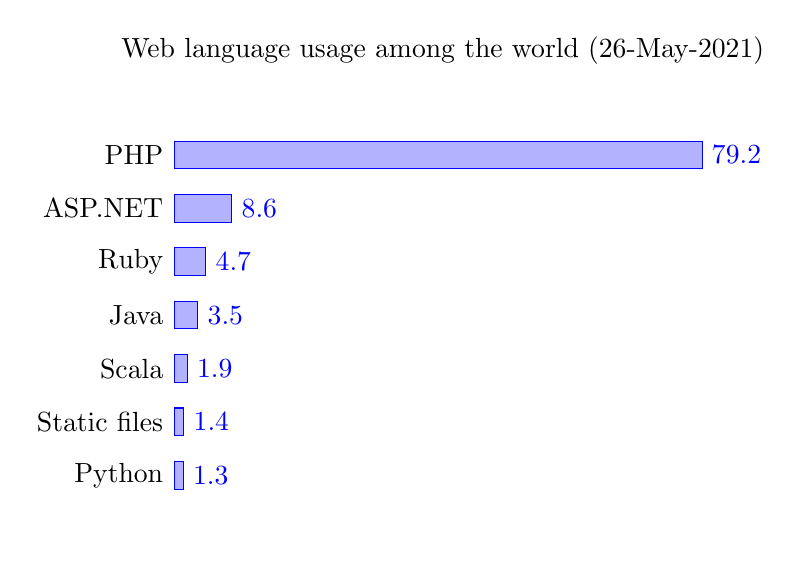
\begin{tikzpicture}
            \begin{axis}[title  = Web language usage among the world (26-May-2021),
                xbar,
                y axis line style = { opacity = 0 },
                axis x line       = none,
                tickwidth         = 0pt,
                ytick             = data,
                enlarge y limits  = 0.2,
                enlarge x limits  = 0.02,
                symbolic y coords = {Python, Static files, Scala, Java, Ruby, ASP.NET,  PHP},
                nodes near coords,
            ]
                \addplot coordinates { (79.2,PHP)         (8.6,ASP.NET)
                (4.7,Ruby)  (3.5,Java) (1.9,Scala) (1.4,Static files) (1.3,Python) };
            \end{axis}
        \end{tikzpicture}

        \url{https://w3techs.com/technologies/overview/programming_language}

        \subsubsection[Docker]{Docker}

        \begin{center}
            
\includegraphics[scale=0.3]{logo_docker}
        \end{center}

        \begin{flushleft}
            Regarding the docker decision, there wasn't much to think about, since docker is a modern technology which I
            already knew the bases, making it easier to pick up and start working earlier.
        \end{flushleft}

        \subsubsection[Docker-compose]{DockerCompose}

        \begin{center}
            
\includegraphics[scale=0.4]{logo_docker_compose}
        \end{center}

        \begin{flushleft}
            This tool facilitates deploying services on a server, while also being able to scalate the services or
            deploy them in a swarm, so there was no excuse to avoid its usage.
        \end{flushleft}

        \newpage
        \subsubsection[Portainer]{Portainer}

        \begin{center}
            
\includegraphics[scale=0.2]{logo_docker_portainer}
        \end{center}

        \begin{flushleft}
            Taking a look at different monitoring tools, decided to use docker portainer mainly by it's fast set-up.
            While still being up to the tasks demanded, which consist in monitoring and managing.
        \end{flushleft}

        \subsubsection[GitHub]{GitHub}

        \begin{center}
            
\includegraphics[scale=0.045]{logo_github}
        \end{center}

        \begin{flushleft}
            On the other hand, I decided to use GitHub to store the project mainly due having a basic understanding of how
            the tools work, since there are multiple tools that suits the same function, felt like that was the right decision.
        \end{flushleft}



        \newpage
        \subsubsection[PostgreSQL]{PostgresSQL}

        \begin{center}
            
\includegraphics[scale=0.3]{logo_postgresql}
        \end{center}

        \begin{flushleft}
            Meanwhile the web language was picked based on its global usage, I personally already have experience with
            Oracle, MySQL, MariaDB and MongoDB, so in order to try a different technology, I decided to use PostgreSQL,
            since it suited my needs while also learning a new database, yet, its position among the ranking, made the
            decision easier to take.
        \end{flushleft}

        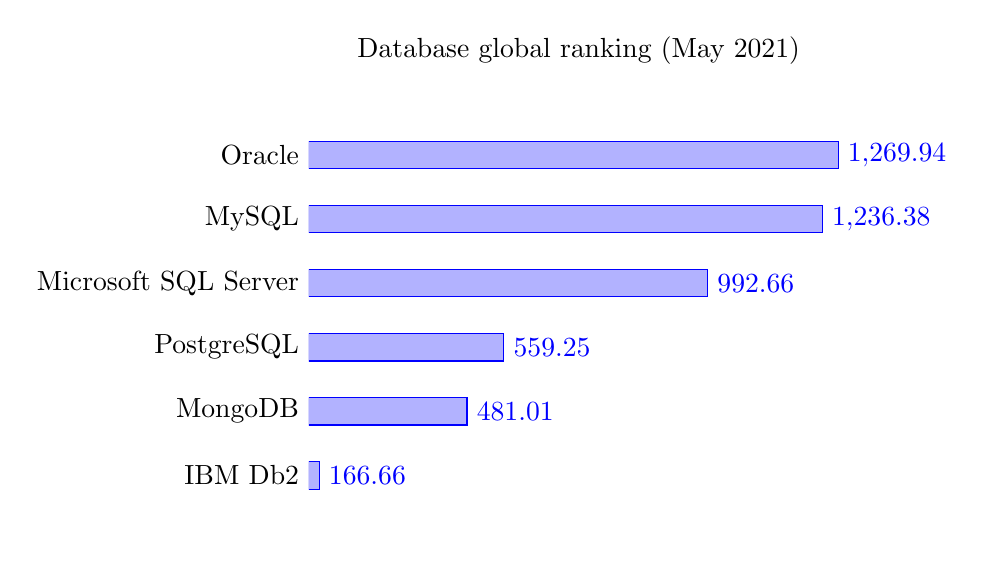
\begin{tikzpicture}
            \begin{axis}[title  = Database global ranking (May 2021),
            xbar,
            y axis line style = { opacity = 0 },
            axis x line       = none,
            tickwidth         = 0pt,
            ytick             = data,
            enlarge y limits  = 0.2,
            enlarge x limits  = 0.02,
            symbolic y coords = {IBM Db2, MongoDB, PostgreSQL, Microsoft SQL Server, MySQL,  Oracle},
            nodes near coords,
            ]
            \addplot coordinates { (1269.94,Oracle)         (1236.38,MySQL)
            (992.66 ,Microsoft SQL Server)  (559.25,PostgreSQL) (481.01,MongoDB) (166.66,IBM Db2) };
            \end{axis}
         \end{tikzpicture}

        \url{https://db-engines.com/en/ranking}

        \subsubsection[Nginx]{Nginx}

        \begin{center}
            
\includegraphics[scale=0.3]{logo_nginx}
        \end{center}
        \begin{flushleft}
            So far, being the main two options Apache and Nginx, I was quite limited when it came to variety,
            and yet, both suit its job very well, yet, due its minor differences, decided to use Nginx instead of Apache,
            since its less resource hungry while being more configurable-wise.
        \end{flushleft}

        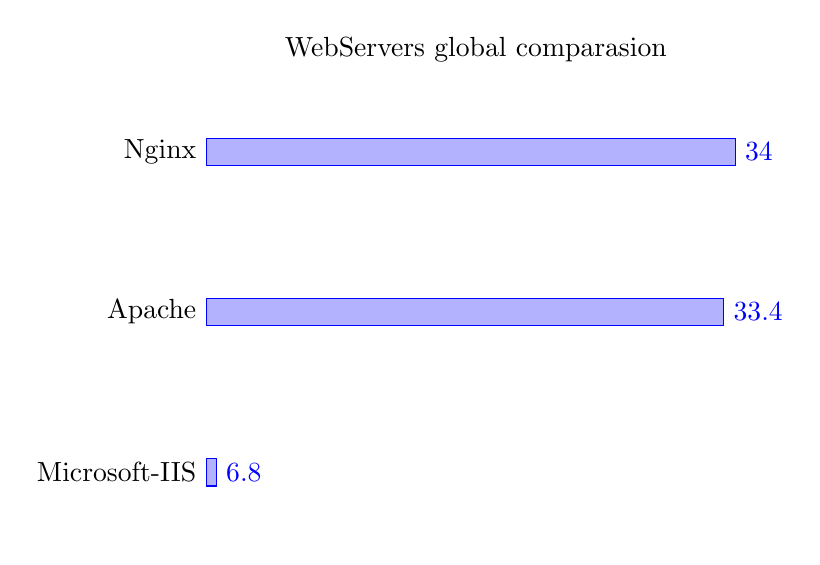
\begin{tikzpicture}
            \begin{axis}[title  = WebServers global comparasion,
            xbar,
            y axis line style = { opacity = 0 },
            axis x line       = none,
            tickwidth         = 0pt,
            ytick             = data,
            enlarge y limits  = 0.2,
            enlarge x limits  = 0.02,
            symbolic y coords = {Microsoft-IIS, Apache, Nginx},
            nodes near coords,
            ]
            \addplot coordinates { (34.0,Nginx) (33.4,Apache) (6.8 ,Microsoft-IIS)};
            \end{axis}
        \end{tikzpicture}

        \begin{flushleft}
            \url{https://w3techs.com/technologies/comparison/ws-apache,ws-microsoftiis,ws-nginx}
        \end{flushleft}

%    Project structure

    \section{Docker Network Scheme}\label{sec:DockerNetworkScheme}
        \subsection{Docker Network Scheme}\label{subsec:ProjectNetworkScheme}
    \begin{center}
    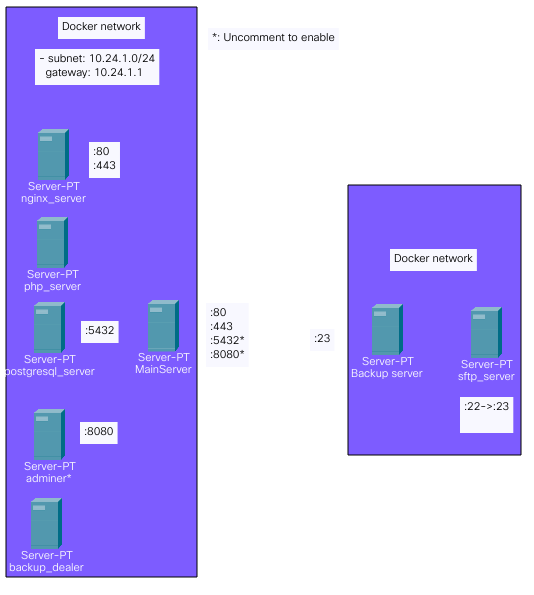
\includegraphics[scale=0.8]{NetworkDistribution}
    \end{center}
    \newpage

    \subsection{Docker Network Distribution Explanation}\label{subsec:dockernetworkdistribution-explanation}
    \begin{flushleft}
        As mentioned previously, the services are distributed in two servers, yet, the second one (the backup server),
        could be removed and store the backups locally, moving the \textbf{sftp} service to the main server, or, through
        \textbf{docker} using a volume or directory binding, but even if it's possible, it's recommended to do the backups in a
        different server as a security measure in case the main server get compromised.
    \end{flushleft}

    \begin{flushleft}
        Taking a look in the main server, we can see that the docker machines are mainly distributed among a common network,
        while there still an \textbf{docker} machine hanging by himself, that's because this \textbf{docker} machine is
        used to generate backups periodically, so doesn't need to have access to another docker networks (unless we wanted to specifically upload
        the backups inside a docker-machine that resides inside a docker network, but we didn't have the need
        to publish the ports in the main server, which is not the actual scenario, nor likely to happen).
    \end{flushleft}


    \subsubsection[Nginx]{Nginx}
    \begin{flushleft}
        Having the ports 80 and 443 exposed in the server, its configuration forces the use of the port 443, redirecting
        the connections fo that port, that way in case of having an HTTP petition the client is forced to use a "secure"
        connection, or at least, a connection that uses SSL encrypting.
    \end{flushleft}

    \subsubsection[PHP]{SFTP}
    \begin{flushleft}
        While this container doesn't do nothing by themself, either has ports exposed, it's linked to the nginx server, providing php support
        to that container.
    \end{flushleft}

    \subsubsection[Postgresql]{Postgresql}
    \begin{flushleft}
        PostgreSQL uses by default the port 5432 to connect to the databases, and while there could be some reasons to
        have it exposed, but since in this scenario we aren't making use of it, it's better to keep it closed, that way
        the connections are limited to the docker machines themselves.
    \end{flushleft}
    \newpage
    \subsubsection[Adminer]{Adminer}
    \begin{flushleft}
        Like previously mentioned, the ports from the database are not exposed, but, in case of needing a simple GUI
        access to them, this can be arranged by using the adminer docker, which provides a web-database management,
        and since it's in the same docker network than the postgresql database, we can have access to it without having
        to expose the ports.
        The active configuration allows you to access the service using the port 8080.
    \end{flushleft}

    \subsubsection[Portainer]{Portainer}
    \begin{flushleft}
        To provide easy access to monitor and control the docker volumes, have decided to implement \textbf{Portainer}
        to the docker network, allowing the users to access to it using the port 9000.
    \end{flushleft}


    \subsubsection[Backup\_dealer]{BackupDealer}
    \begin{flushleft}
       Like mentioned previously, this machine is used to periodically do backups of the desired volumes or directories,
       to a local volume or directory, or to a remote server.
       There isn't much to talk about it, since it doesn't provide a service by himself.
    \end{flushleft}

    \subsubsection[SFTP]{SFTP}
    \begin{flushleft}
        Observing the schema, we can see that the port 22 is being forwarded to the port 23, and publishing it, that's
        to avoid a port overlap with the default SSH port configuration.
    \end{flushleft}



    \newpage
    \subsection[Main Server Docker Configuration]{MainServerDockerConfiguration}\label{subsec:mainserverdockerconfiguration}
    \subsubsection[Main Server Docker-Compose]{Main Server DockerCompose}
    \lstinputlisting[language=Yaml,label={lst:MainDockerCompose}]{../docker-compose.yml}
    \paragraph{docker-compose.yml} that contains the services for the main server.
    \newpage
    \begin{flushleft}
        The main things worth to mention, besides the open ports which are already commented (yet again will be listed here),
        it's the restart policies and pointing out which services need to be build instead of using a raw image.
    \end{flushleft}
    \begin{enumerate}
        \item Networks:
            \begin{itemize}
                \item shop\_net:
                \begin{itemize}
                    \item nginx
                    \item php
                    \item adminer
                    \item postgresql
                \end{itemize}
                \item agent\_network:
                \begin{itemize}
                    \item portainer
                \end{itemize}
            \end{itemize}
        \item Volumes
            \begin{itemize}
                \item postgresql\_volume:
                \begin{itemize}
                      \item postgresql
                \end{itemize}
                \item portainer\_data:
                \begin{itemize}
                      \item portainer
                \end{itemize}
            \end{itemize}

    \end{enumerate}

    \begin{flushleft}
        All the dockers have been configured to restart in case of failure, which means that unless they are stopped manually,
        they will always restart.
    \end{flushleft}
    \begin{flushleft}
        Also, as will be explained in the next section, the services PHP and PostgreSQL, are being built fromm
    \end{flushleft}

    \subsubsection[PHP Dockerfile]{PHP Dockerfile}
    \lstinputlisting[language=Yaml,label={lst:BackupDealer}]{../Dockerfiles/php}


    \newpage
%    Service Configuration
    \section{Services Configuration}\label{sec:ServicesConfiguration}
%    Docker Config
    \subsection[Docker Configuration]{DockerConfiguration}\label{subsec:dockerconfiguration}
    \subsubsection[Main Server Docker Configuration]{MainServerDockerConfiguration}
    \
    \lstinputlisting[language=Yaml,label={lst:MainDockerCompose}]{../docker-compose.yml}












    \section{Services Deployment}\label{sec:ServiceDeployment}
\end{document}